\documentclass[
        a4paper,
        10pt,
        parskip = full,    % Layout with zero \parident and non-zero \parskip
    ]{scrartcl}
% \usepackage[utf8]{inputenc}

\usepackage[top=2cm, bottom=2.5cm, left=2.5cm, right=2.5cm]{geometry}
\usepackage[
        colorlinks = true,    % Disable drawing boxes around links.
        linkcolor = black,    % Sets the color of links to black.
    ]{hyperref}
\usepackage{amsmath}
\usepackage{graphicx}
\usepackage{subfig}
\usepackage{float}

\begin{document}

\textbf{\large{Laboratory - Deep Learning Lab, WS 2018/2019 - Exercise 4}}

\textbf{\large{Submitted by:\\
\\
Amadeus Hovekamp,\\
mail@amadeus-hovekamp.de,\\
Matr. no: 4603934\\
\\
Hans Nübel,\\
hans.nuebel@rwth-aachen.de,\\
Matr. no: 4514598}}

The repository with the source code can be found under the following link:\\
\href{https://github.com/Schokokugel/RoboticsLab}
     {https://github.com/Schokokugel/RoboticsLab}


\section{Getting Set Up}

As the set up for this exercise was the same as for the last exercise, there were no issues here.

\section{Reinforcement Learning: Deep Q-Networks}

\subsection{CartPole}

All in all the implementation of the DQN went well, the provided components
helped to implement it. We implemented some additional features that helped us
training the network and generating the required data for generating the report.


The first runs were not successfull due to the small default learning
rate of 0.0001. Changing the learning rate to 0.001 lead to good results,
which can be seen in the following figures \ref{CartPoleTrainEvalReward}
and \ref{CartPoleTestReward}.


The total run had a length of 500 episodes, the reward for each episode is
displayed by the dots in figure~\ref{CartPoleTrainEvalReward}. The orange line
shows the evaluation reward after every tenth episode, averaged over 5 evaluation
runs using only deterministic actions.

It took the agent about 120 episodes to learn how to prevent the pole from tilting
but still drove off to the side quickly. After 180 it was sometimes able to
balance the pole for the complete episode consisting of 1000 steps. 40 episodes
later it managed to do so consistently. Somewhat suprisingly it $unlearned$ to
how balance the pole after 60 episodes later. This could be due to more and more
of the same states (the pole is almost upright, neither cart or the pole move much)
filling up the replay buffer and thus overfitting the network to highly similar
states. This would also explain the learning-unlearning oszillations later on.
A hint in the source code defined the task as $solved$ when the average reward is
greater than or equal to 195.0 over 100 consecutive trials, which was reached
after 170 episodes.

Figure~\ref{CartPoleTestReward} shows the test rewards achieved with the trained
networks over 15 episodes, once where the network was trained until it is
conisdered as solved, and once after training for the full run of 500 episodes.
It is visible, that the longer trained network achieved better results.

\begin{figure}[H]
  \begin{center}
    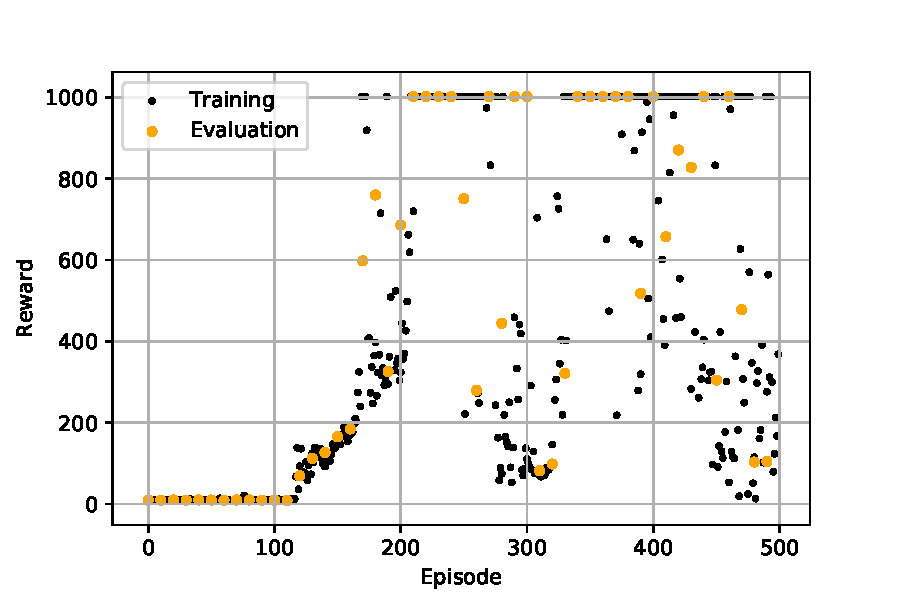
\includegraphics{./images/CartPole-v0/tb_train_eval_reward.pdf}
    \caption{CartPole - Episode Reward during Training}
    \label{CartPoleTrainEvalReward}
  \end{center}
\end{figure}

\begin{figure}[H]
  \begin{center}
    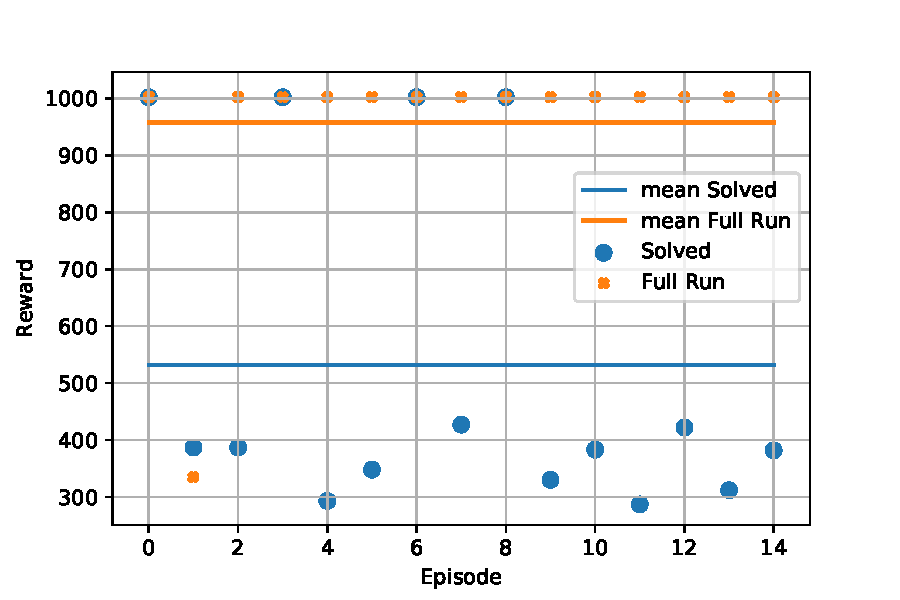
\includegraphics{./images/CartPole-v0/tb_test_reward.pdf}
    \caption{CartPole - Episode Reward for Testing}
    \label{CartPoleTestReward}
  \end{center}
\end{figure}


\subsection{MountainCar}

For the MountainCar environment we used the same setup and network as for the
CartPole environment, leading also to good results, which are displayed in the
figures~\ref{MountainCarTrainEvalReward} and~\ref{MountainCarTestReward}.

\begin{figure}[H]
  \begin{center}
    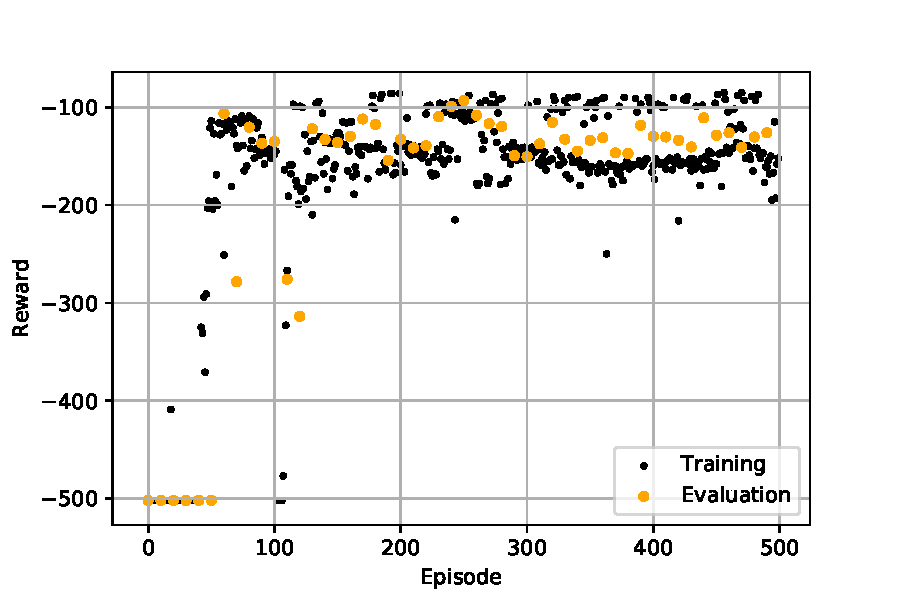
\includegraphics{./images/MountainCar-v0/tb_train_eval_reward.pdf}
    \caption{MountainCar - Episode Reward during Training}
    \label{MountainCarTrainEvalReward}
  \end{center}
\end{figure}

In figure~\ref{MountainCarTrainEvalReward} the training and evaluation rewards
are displayed as in the CartPole environment. Here, already after 60
episodes the network performs good. But later on again an oscillation behavior
can be seen, though the bad performances are not dropping are not getting as bad
as some performances for the CartPole. A reason for this difference is probably
that the CartPole is more difficult, consisting of two tasks at the same time
(balancing the pole and not drifting off to the side).

Finally, in figure~\ref{MountainCarTestReward} the test rewards for the
solved model and the full run model are displayed. Here, we have defined solved
as reaching an average score larger than -200 over 100 consecutive runs,
similar so the definition as for the CartPole. In contrast to the CartPole,
Solved scores higher on average but the Full Run, which is in turn better when
the starting conditions are favorable for its risky driving style trying to
minimize drives trough the valley.

\begin{figure}[H]
  \begin{center}
    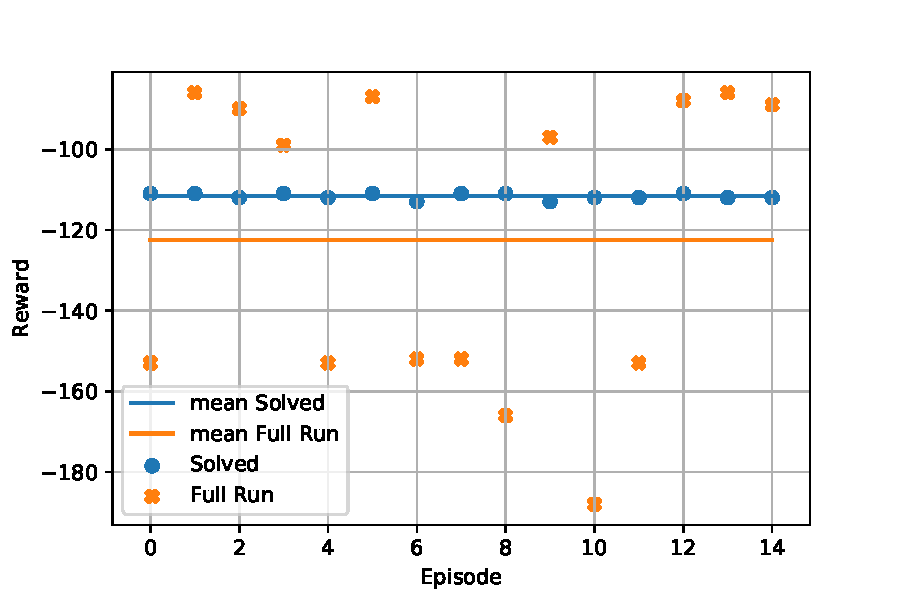
\includegraphics{./images/MountainCar-v0/tb_test_reward.pdf}
    \caption{MountainCar - Episode Reward for Testing}
    \label{MountainCarTestReward}
  \end{center}
\end{figure}






\subsection{CarRacing}

\subsubsection{The network structure}
We used a CCN that consists of two convolution layers (20 filters, 11 kernel size, stride 1), each followed by a max
pooling (first: pool\_size 2, stride 2; second: pool\_size 2, stride 1) and a fully connected
layer (128 units). The input layer size is 98 by 98 by history\_length and output layer with 5 units.


\begin{center}
    \begin{tabular}{ | l | l | l | l | l | l | l | l |}
    \hline
                            & \textbf{1st run} & \textbf{2nd run} & \textbf{3rd run} &
                            \textbf{4th run} & \textbf{5th run} & \textbf{6th run} & \textbf{7th run} \\ \hline
    \textbf{epsilon}        &  0.2  &  0.15  &  0.1  &  0.05  &  0.04  &  0.03  &  0.05  \\ \hline
    \textbf{max\_timesteps} &  150  &  200   &  300  &  300   &  450   &  700   &  1000  \\ \hline
    \end{tabular}
\end{center}

\begin{figure}[H]
  \begin{center}
    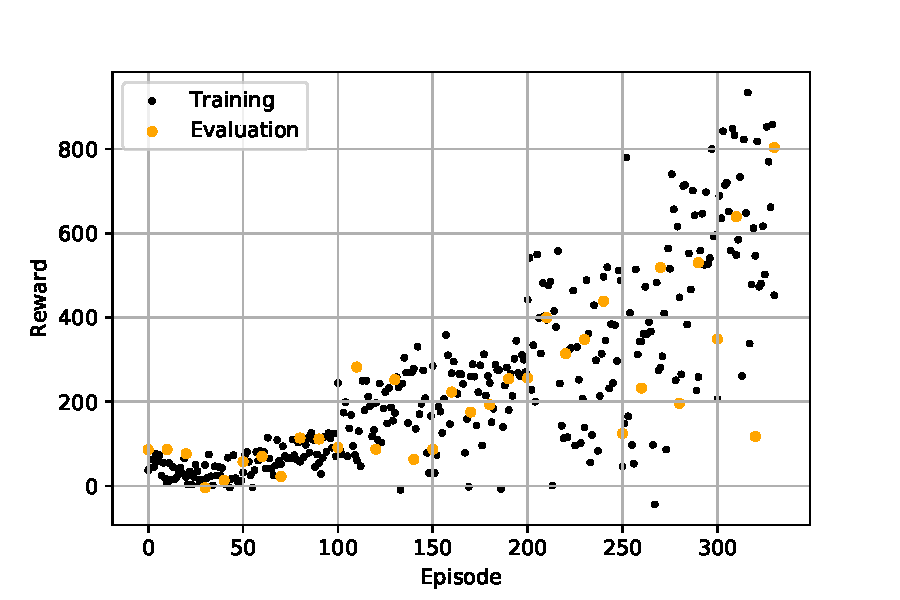
\includegraphics{./images/CarRacing-v0/tb_train_eval_reward.pdf}
    \caption{CarRacing - Episode Reward during Training}
    \label{CarRacingTrainEvalReward}
  \end{center}
\end{figure}

\begin{figure}[H]
  \begin{center}
    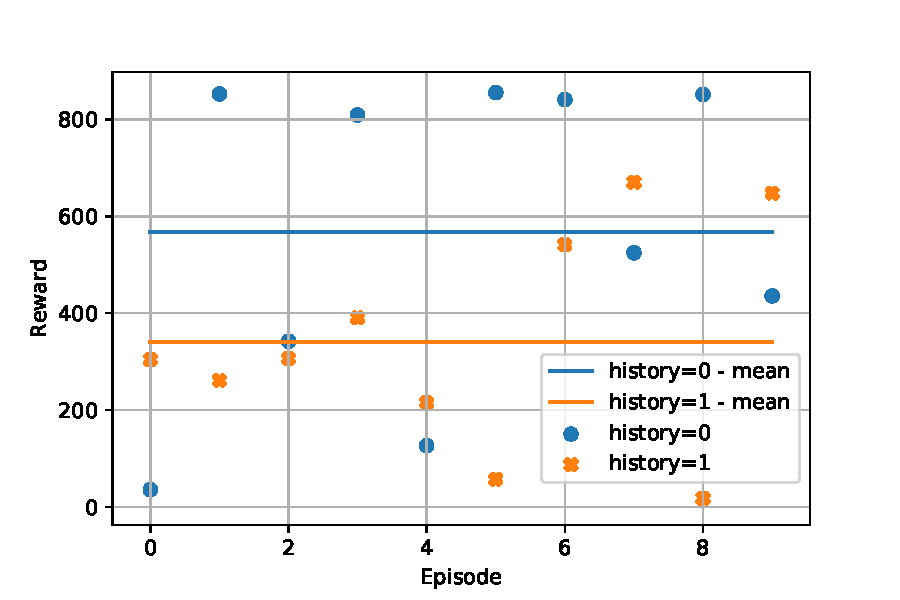
\includegraphics{./images/CarRacing-v0/tb_test_reward.pdf}
    \caption{CarRacing - Episode Reward for Testing}
    \label{CarRacingTestReward}
  \end{center}
\end{figure}


\subsection{An improved network}


\section{Influence of hyperparameters}

\end{document}
